\documentclass[a4paper, 11pt]{article}
\usepackage{amsmath}
\usepackage{graphicx}
\usepackage{geometry}
\usepackage{listings}
\usepackage{xcolor}
\usepackage{float}
\usepackage[fontset=ubuntu]{ctex}
\geometry{scale=0.8}
\linespread{1.5}
\usepackage{hyperref}

\lstset{
    %backgroundcolor=\color{red!50!green!50!blue!50},%代码块背景色为浅灰色
    rulesepcolor= \color{gray}, %代码块边框颜色
    breaklines=true,  %代码过长则换行
    numbers=left, %行号在左侧显示
    numberstyle= \small,%行号字体
    %keywordstyle= \color{blue},%关键字颜色
    commentstyle=\color{gray}, %注释颜色
    frame=shadowbox%用方框框住代码块
    }



\title{	
\normalfont \normalsize
\textsc{School of Data and Computer Science, Sun Yat-sen University} \\ [25pt] %textsc small capital letters
\rule{\textwidth}{0.5pt} \\[0.4cm] % Thin top horizontal rule
\huge  prolog  简介 \\ % The assignment title
\rule{\textwidth}{2pt} \\[0.5cm] % Thick bottom horizontal rule
\date{\normalsize October 1, 2020} 
}

\begin{document}
\maketitle
\tableofcontents
\newpage

\section{prolog 简介}
Prolog 是一种逻辑编程语言。它创建在逻辑学的理论基础之上,最初被运用于自然语言等研究领域。现在它已广泛的应用在人工智能的研究中,它可以用来建造专家系统,自然语言理解,智能知识库等。

目前来说,Prolog主要用在人工智能和计算机语言的研究领域。有别于一般的过编程语言,prolog的程式是基于谓词逻辑的理论。最基本的写法是定立物件与物件之间的关系,之后可以用询问目标的方式来查询各种物件之间的关系。系统会自动进行匹配及回溯,找出所询问的答案。

\section{prolog 安装}
具体下载可去https://www.swi-prolog.org/Download.html下载安装,根据系统不同自行选择。
\begin{figure}[ht]
\centering

\includegraphics[scale=0.6]{E05_2019096_Family/prolog introduction/pic/download.png}
\caption{根据不同系统自行选择}
\label{fig:label}
\end{figure}

\section{prolog 语法}
\subsection{启动 prolog}
Linux 和 Mac 都可以通过在控制台输入swipl启动prolog,window系统在搜索框输入prolog,点击图标即可进入。当你看到 ?- 的时候,你就成功了。

\colorbox{pink}{\color{black} ?- }是命令提示符,我们来看一个例子:
\begin{figure}[ht]
\centering
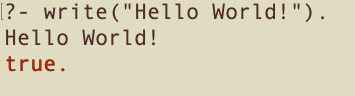
\includegraphics[scale=0.6]{E05_2019096_Family/prolog introduction/pic/code1.png}
\label{fig:label}
\end{figure}

prolog所有的语句都会用\colorbox{pink}{\color{black} . }
来标识结束。如果想要换行,可以在中间加入\colorbox{pink}{\color{black} nl }。
\begin{figure}[ht]
\centering
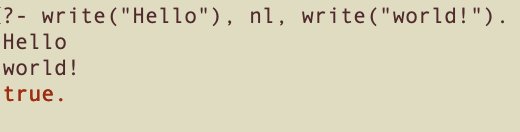
\includegraphics[scale=0.6]{E05_2019096_Family/prolog introduction/pic/code2.png}
\label{fig:label}
\end{figure}
退出可以使用\colorbox{pink}{\color{black} halt }命令。

\subsection{常量,变量}
小写字符串开头的就是常量,大写字符开头的就是变量,如:
\colorbox{pink}{\color{black} abc },这是常量。
\colorbox{pink}{\color{black} Abc },这是变量。
\begin{figure}[ht]
\centering
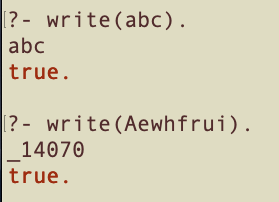
\includegraphics[scale=0.6]{E05_2019096_Family/prolog introduction/pic/code3.png}
\label{fig:label}
\end{figure}

\subsection{关系,属性}
两个常量之间的关系,我们可以使用小括号来标识,如mike是jack是爸爸,可以表示成:\colorbox{pink}{\color{black} father(mike, jack). },这只是单方面的关系,反过来是不一定成立的。\colorbox{pink}{\color{black} friend(x, y). }x是y的朋友,但y不一定是x的朋友(至少prolog不这么认为)。如果要用frind来表达x,y是朋友,则需要写两遍了。\colorbox{pink}{\color{black} friend(x, y). friend(y, x). }

两个常量之间是用小括号表达,但是如果是只有一个参数,那就表示该常量拥有这个属性。如\colorbox{pink}{\color{black} male(jack).},jack拥有男性这个属性。

\subsection{规则}
规则也就是推理的依据,我们可以根据规则从一个已有的结论推理出另外一个结论。
如x和y是朋友,我们需要重复两遍:
\begin{figure}[ht]
\centering
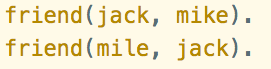
\includegraphics[scale=0.6]{E05_2019096_Family/prolog introduction/pic/code4.png}
\label{fig:label}
\end{figure}

如果使用规则,我们可以写成:

\begin{figure}[ht]
\centering
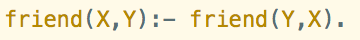
\includegraphics[scale=0.6]{E05_2019096_Family/prolog introduction/pic/code5.png}
\label{fig:label}
\end{figure}


上述代码的\colorbox{pink}{\color{black} X,Y}都是大写,所以是变量,符号\colorbox{pink}{\color{black} :-}代表了推理关系,和蕴含\colorbox{pink}{\color{black} <-}意思相同,只要右边表达式为真,左边就可以满足。所以如果加上这条规则,只需要写\colorbox{pink}{\color{black} friend(jack, mike). }就可以表示jack和mike是朋友了。
如果一条规则需要应用多个判断条件,如表示\colorbox{pink}{\color{black} X}是\colorbox{pink}{\color{black} Y}的儿子:


\begin{figure}[H]
\centering

\includegraphics[scale=0.6]{E05_2019096_Family/prolog introduction/pic/code6.png}
\label{fig:label}
\end{figure}


\colorbox{pink}{\color{black} X}是\colorbox{pink}{\color{black} Y}的儿子首先要求\colorbox{pink}{\color{black} X}是男生,其次\colorbox{pink}{\color{black} Y}可能是\colorbox{pink}{\color{black} X}的父亲也可能是母亲,这里就存在了一个或的关系。在prolog中,我们使用\colorbox{pink}{\color{black} ,}和\colorbox{pink}{\color{black} ;}表达“且”和“或”的关系。

如果我们需要对某个条件做否定,比如我们定义单相思,相思用谓语\colorbox{pink}{\color{black} love(X,Y).}来定义。于是单相思可以定义成:
\begin{figure}[H]
\centering
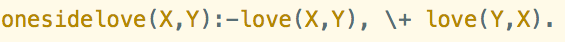
\includegraphics[scale=0.6]{E05_2019096_Family/prolog introduction/pic/code7.png}
\label{fig:label}
\end{figure}
其中,\colorbox{pink}{\color{black} $\backslash$+}后面紧跟的条件如果是false才能匹配当前的规则。

\subsection{比较}
我们需要知道两个比较操作符号 \colorbox{pink}{\color{black} =} 和 \colorbox{pink}{\color{black} $\backslash$=}
\begin{lstlisting}[language={java}]
X = a, X = b.
X = a, Y = X.
\end{lstlisting}

第一个会返回false。如果变量没有被初始化,而等号的另一边是常量,这个时候常量就会赋值给变量;如果变量已经被初始化完成了,那么等号就会起比较的作用了。X = a中X没有被赋值,所以X = a相当于把a赋值给X。X = b要执行时X已经被a赋值了,所以等于号起了比较的作业,X = b返回false。


第二个返回Y = a,相当于是赋值,首先X没有被初始化,所以X会被赋值a,Y也没有被初始化,而X被初始化了,Y也被初始化成了a。

\begin{lstlisting}[language={java}]
X = a, X \= a.
\end{lstlisting}

返回 false, 'X = a' 会把a赋值给X, 然后对比X和a,\colorbox{pink}{\color{black} $\backslash$=}表示如果不等则返回true。

\subsection{Setof}
现在存在一个知识库如下所示。

\begin{lstlisting}[language={java}]
age(peter, 7).
age(ann, 5).
age(pat, 8).
age(tom, 5).
age(ann, 5).

like(jack, ann).
age(X, 8) :- like(X, ann).
\end{lstlisting}

我们可以使用\colorbox{pink}{\color{black} Setof} 来获取所有具有Age属性的孩子.(也 age(X, Y).)
\begin{lstlisting}[language={prolog}]
?- setof(Child, age(Child, Age), Results).
Age = 5,
Results = [ann, tom] ;
Age = 7,
Results = [peter] ;
Age = 8,
Results = [jack, pat].
\end{lstlisting}

任何出现在“age(Child, Age)”中的变量(如Child,Age),那个没有出现在第一个参数变量里面的(如Age),“setof”会根据这个参数返回所有的可能性。

我们可以通过另外一种方式完成:
\begin{lstlisting}[language={prolog}]
?- setof(Age/Child, age(Child, Age), Results).
Results = [5/ann, 5/tom, 7/peter, 8/jack, 8/pat].
\end{lstlisting}

如果我们不关心分类,只想返回所有的结果。
\begin{lstlisting}[language={prolog}]
?- setof(Child, Age^age(Child, Age), Results).
Results = [ann, jack, pat, peter, tom].
\end{lstlisting}

可以解释成:我们要寻找所有具有年龄属性的孩子,并把结果放到Results中。



\subsection{查询}
规则既然已经定义好了,那我们就应该把规则导进来。
先写好一个脚本\colorbox{pink}{\color{black} rules.pl},然后通过\colorbox{pink}{\color{black} ?- [rules]}导入脚本。(如果你不知道你的prolog默认读取文件的路径,可以用\colorbox{pink}{\color{black} ?- pwd}查看路径)

\begin{figure}[H]
\centering
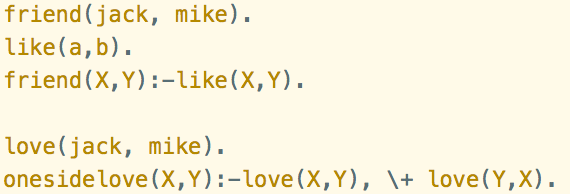
\includegraphics[scale=0.6]{E05_2019096_Family/prolog introduction/pic/code8.png}
\caption{rules.pl内容}
\end{figure}

\begin{figure}[H]
\centering
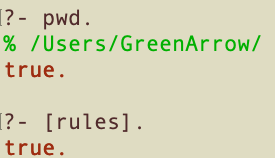
\includegraphics[scale=0.6]{E05_2019096_Family/prolog introduction/pic/code9.png}
\label{fig:label}
\caption{先查看prolog默认文件路径,把rules.pl放置到该路径下,再用[rules]命令读取}
\end{figure}

接下来我们查询即可。
\begin{figure}[H]
\centering
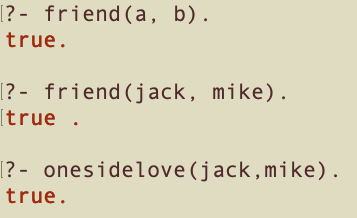
\includegraphics[scale=0.6]{E05_2019096_Family/prolog introduction/pic/code10.png}
\end{figure}

返回\colorbox{pink}{\color{black} true.}则说明查找成功。还可以查询jack的朋友有哪些:
\begin{figure}[H]
\centering
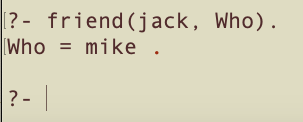
\includegraphics[scale=0.6]{E05_2019096_Family/prolog introduction/pic/code11.png}
\end{figure}

\section{样例}
\subsection{阶乘}
\begin{lstlisting}[language={java}]
factorial(N){
    if(N == 0 || N == 1) return 1;
    return factorial(N-1) * N;
}
\end{lstlisting}
首先,我们要给出初始条件,当N为1或者是0时需要返回1。

\begin{lstlisting}[language={java}]
factorial(1, 1).
factorial(0, 1).
\end{lstlisting}

当 \colorbox{pink}{\color{black} N > 1}, \colorbox{pink}{\color{black} N = N - 1}, 返回 \colorbox{pink}{\color{black} N * factorial(N-1)}. 但这里是 factorial(N, Return), prolog没有返回,所以我们需要先计算  \colorbox{pink}{\color{black} factorial(N-1, Return1)},然后\colorbox{pink}{\color{black} Return = Return1 * N}.
\begin{lstlisting}[language={java}]
factorial(N,Ret) :-  N > 1, N1 is N - 1, factorial(N1, Ret1), Ret is N * Ret1.
\end{lstlisting}

\subsection{Fibonacci}
\begin{lstlisting}[language={java}]
fibonacci(N){
    if(N == 1 || N == 2) return 1;
    return fibonacci(N-1) + fibonacci(N-2);
}
\end{lstlisting}

相似的,我们先给出初始条件。
\begin{lstlisting}[language={java}]
fibonacci(1, 1).
fibonacci(2, 1).
\end{lstlisting}

当 \colorbox{pink}{\color{black} N > 2},  fibonacci(N-1) + fibonacci(N-2), 但这里是  fibonacci(N, return), N1 = N-1, N2 = N-2, 先计算  fibonacci(N1, Return1) 和 fibonacci(N2, Return2) 得到 Return1 和 Return2, Return = Return1 + Return2。

\begin{lstlisting}[language={prolog}]
fib(N,Ret) :- N > 2, N1 is N -1, N2 is N -2, fib(N1,Prv1), fib(N2,Prv2), Ret is Prv2 + Prv1.
\end{lstlisting}

如果 N > 2, 然后计算 fib(N1,Prv1), fib(N2,Prv2). Ret = Prv2 + Prv1就是最后的结果。

\subsection{Hanio}
\begin{lstlisting}[language={java}]
move(N, A, B, C){
    if(N==1){
       move A to C;
    }
    else
    {
        move(N-1,A,C,B);
        move A to C;
        move(N-1,B,A,C);
    }
}
\end{lstlisting}

如果 N == 1, 我们可以直接把物体从A移动到C,不需要借助任何东西。但如果 N > 1, 我们必须首先把N-1个物体借助C从A移动到B, 然后把最后一个物体直接从A移动到C.最后,重新把N-1个物体从B借助A移动到C。

定义要解决的物体:
\begin{lstlisting}[language={prolog}]
hanio(N) :- move(N, a, b, c).
\end{lstlisting}

我们应该把N个物体从A移动到C。

特别的,
\begin{lstlisting}[language={prolog}]
move(1,A,_,C):-inform(A,C).
\end{lstlisting}

当只有一个物体,我们不需要借助任何东西就可以直接从A移动到C。

\begin{lstlisting}[language={prolog}]
move(N,A,B,C):-N1 is N-1,move(N1,A,C,B),inform(A,C),move(N1,B,A,C).
\end{lstlisting}

下一步,我们将N-1个物体从A移动到B借助C (\colorbox{pink}{\color{black} move(N1,A,C,B)}), 然后把最后一个从A移动到C(\colorbox{pink}{\color{black} inform(A,C)}), 最后又重新把N-1个物体从B移动回C(\colorbox{pink}{\color{black} move(N1,B,A,C)}).

定义 inform函数:
\begin{lstlisting}[language={prolog}]
inform(Loc1,Loc2):-nl,write('from '),write(Loc1),write(' to '),write(Loc2).
\end{lstlisting}


%\clearpage
%\bibliography{E:/Papers/LiuLab}
%\bibliographystyle{apalike}
\end{document} 
%%% Local Variables:
%%% mode: latex
%%% TeX-master: t
%%% End:
\documentclass[a4paper, 11pt]{article}
\usepackage{amsmath}
\usepackage{graphicx}
\usepackage{geometry}
\usepackage{listings}
\geometry{scale=0.8}
\linespread{1.5}
\usepackage{hyperref}





%%% Local Variables:
%%% mode: latex
%%% TeX-master: t
%%% End:
